\section{Spectral Shape Estimation}
\label{sec:methods}

We approached the problem of estimating radiance distribution curves with machine learning (ML), a superset discipline including much of statistics and neural networks. There are a variety of approaches, algorithms, and software frameworks to choose from. For this work, we focused on a small subset, statistical regression models, and used scikit-learn\cite{pedregosa_scikit}, a powerful, popular open source library written in Python and Cython,\cite{behnel_cython} providing most standard ML functionality (supervised/unsupervised algorithms, $k$-fold cross validation, principal component analysis, imputation, etc.).

We use $k$-fold cross-validation (CV), or rotation estimation,\cite{picard_cv,kohavi_cvstudy} to get the most out of our dataset and to minimize the variance of prediction accuracy. We used 10-fold CV specifically to have larger subsamples and less risk of over-fitting. 0 samples from final test captures were used for training, to avoid bias and data leakage.\cite{cawley_overfitting}

In general there are three primary problem categories in machine learning: classification, regression, and clustering, and three primary learning modes: supervised, unsupervised, and reinforcement. Predicting a radiance distribution, essentially a continuous curve of points, using correlated ground truths, is a supervised regression problem. Thus our first task was clear -  we needed to clean, correlate, and export all usable measurements into datasets of input-output mappings (or samples), each of which correspond to a single directional radiance measurement, and each of which would be used for either CV training/testing or final holdout testing. The initial measured (raw) features extracted from our data include: timestamp, pixel colors $(RGB)$, measurement location $(azimuth, altitude)$, and directional radiance values per wavelength. The use of multiple exposure (HDR) pixel values and sky irradiance were left for future/ongoing work, though it stands to reason that multiple pixel values across multiple images can just as easily be used as features, as a single pixel value.

Next, we determined which parameters were needed for our model. Feature engineering, the process of determining which inputs best represent the correlated outputs, is an important and often time-consuming part of any machine learning project.\cite{mitchell_ml, domingos_feature, forman_feature, brownlee_mlmastery} It is not recommended to rely on raw features alone. Too many features may distract an algorithm, while too few may be insufficient to model complex relationships. Investigative exploratory data analysis (EDA) on the raw features gave us insight and preliminary performance metrics, such as the importance of one feature over another, the insignificance of sample azimuth, etc. Fig. \ref{fig:eda} shows a subset of EDA techniques employed.

%I confirm the same results as Brandon's. Replacing drop out data with taking the average of the column and shifting negative values didn't have any impact on regression score.

\begin{figure} [b]
\begin{center}
\begin{tabular}{c}
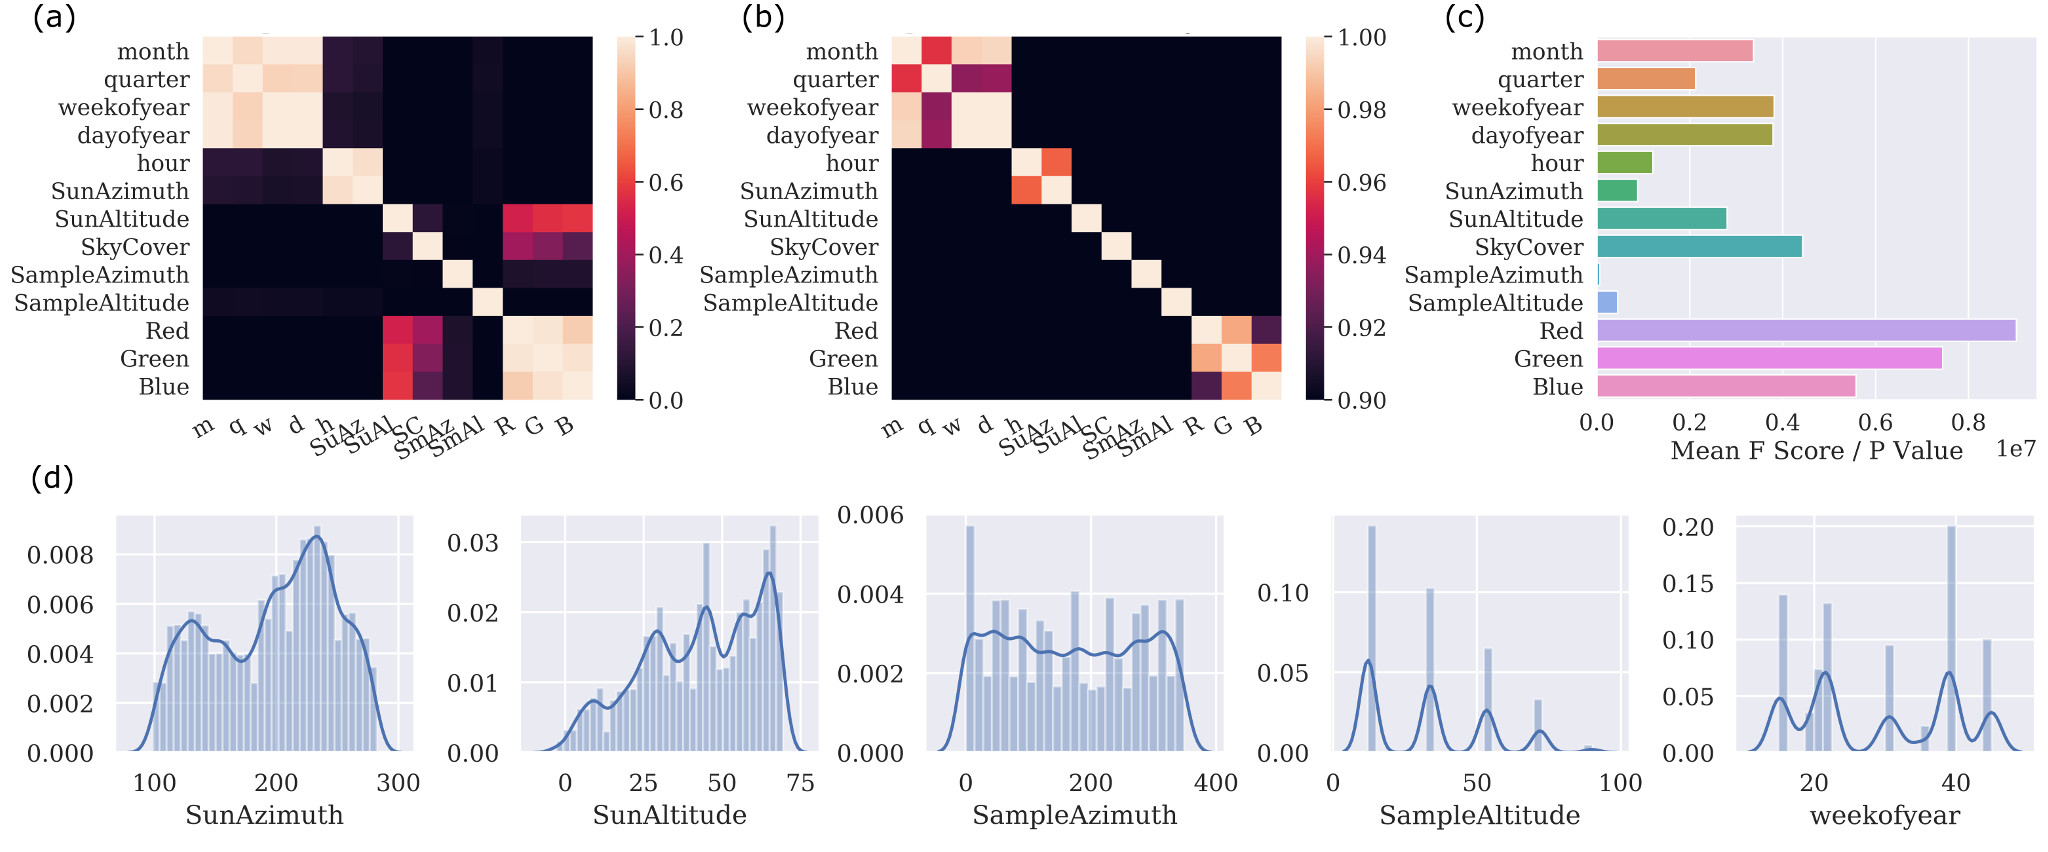
\includegraphics[width=0.98\textwidth]{img/eda.jpg}
\end{tabular}
\end{center}
\caption[eda] { \label{fig:eda}EDA (a) correlation matrix, (b) collinearity matrix, (c) feature importance , and (d) histograms.}
\end{figure}

After EDA, we began searching for an appropriate regression model. Though predicting spectral radiance is clearly a regression problem, it was not so clear which regression model should be used. Many common statistical models (for both regression and classification problems) produce a single output, and thus have high-dimensional input and low-dimensional (i.e. 1) output. We had the exact opposite problem - a handful of input features to predict 2151 values (wavelengths 350-2500nm). Multi-output regression models seemed best suited to the challenge. We started with the simplest possible model as a baseline, the linear regression model (with multi-output support). We refer to this model as LNR. As expected, initial scores were low (since outputs are highly noisy curves, not linear trends), implying under-fitting and the need for more complexity to the inputs.

We accomplished this several ways: (1) by ``binning" the capture timestamp into discretized buckets (quarter, month, week, hour, etc.), (2) by computing the sun's azimuth and zenith/altitude per capture, (3) by tagging samples with sky cover assessment, and (4,5) with polynomial modeling and feature scaling, respectively. In addition to providing a more complex input, method (1) has the benefit of potentially capturing seasonal and daily shifts such as dawn/day/dusk/night, as well as rainy versus arid seasons, all of which have different skies and sometimes trending turbidity.\cite{power_seasonal} Method (2) complies with the motivation for this work, that the sun's zenith/altitude might have a large impact on the shape of a radiance curve. The feature importance graph in Fig.~\ref{fig:eda} confirms this. Summarized by Chauvin et al., when considering radiance at any given point in the sky, of capital importance is the point-to-zenith angle (PZA), the sun-to-zenith angle (SZA), and the central sun-to-point angle (SPA) between them.\cite{chauvin_modelling_2015} We believe the importance of this information is captured by both the measured sample position and computed sun position included in each sample. As mentioned in Sec.~\ref{sec:data}, we used NREL's SPA algorithm for computing sun position per capture.\cite{reda_spa} Method (3) is also discussed in Sec.~\ref{sec:data}. Method (4), polynomial modeling, has been used for decades for problems such as curve fitting.\cite{deboor_splines} We used it to generate a polynomial combination of features from our specified set of inputs along with a polynomial degree (e.g. the set $[a, b]$ becomes $[1, a, b, a^2, ab, b^2]$ with a degree of 2).\cite{pedregosa_scikit} Specifically, we found that using this polynomial modeling technique with a degree of 4 on the inputs of the LNR model, boosted its CV test score considerably. Our final feature engineering contribution, method (5), involved the use of scalers on the inputs: standard, robust, and quantile transformer,\cite{pedregosa_scikit} all of which attempt to spread the input over a uniform distribution and reduce the impact of marginal outliers.\cite{pedregosa_scikit} The quantile transformer in particular had the greatest positive impact, and so we applied, saved, and loaded it alongside our models. After data processing and feature engineering, a final train/test sample consists of the input and output features shown in Fig.~\ref{fig:features}. Future work will include more input features.

\begin{figure} [b]
\begin{center}
\begin{tabular}{c}
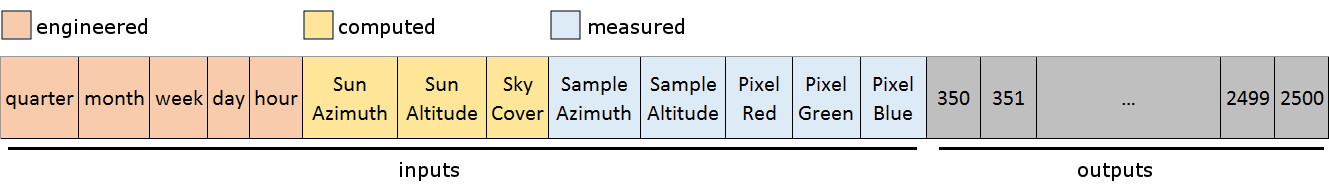
\includegraphics[width=0.98\textwidth]{img/features.jpg}
\end{tabular}
\end{center}
\caption[features] {\label{fig:features}A dataset sample consists of 13 input features and 2151 output features (the radiance curve).}
\end{figure}

We used the following error metrics to compare models and assess prediction performance: coefficient of determination score (R$^2$) and root mean squared deviation (RMSD). We also considered mean bias deviation (MBD), but found it to be ``noisy" without much correlation to R$^2$ and RMSD. We believe this error metric is best suited to a single wavelength, not deviation across a whole curve. The R$^2$ score we used comes from scikit-learn,\cite{pedregosa_scikit} and is defined as:
\begin{equation}
\label{eq:r2}
R^2(x,y) = 1 - \frac{\sum_{i=1}^{N} (x_i-y_i)^2} {\sum_{i=1}^{N} (x_i-\bar{x}_i)^2} ~~\textrm{,}
\end{equation}
where $(x,y)$ is a (truth, prediction) pair, $N$ the number of curves considered, and $\bar{x} = \frac{1}{N}\sum_{i=1}^{N} x_i$~. Note that this score can be negative, despite the name R$^2$. As with Tohsing et al.\cite{tohsing_validation_2014} and others, we used the RMSD metric provided by Iqbal,\cite{iqbal_intro} which indicates the variation of predicted from measured, and is defined as:
\begin{equation}
\label{eq:mbd}
RMSD=\sqrt[]{\frac{\sum_{i=1}^{N} (y_i-x_i)^2}{N}}
\end{equation}
where $N$ is the number of curves considered, $x$ the measured/truth curves, and $y$ the predicted.

\subsection{Machine Learning Models}

After feature engineering and preliminary tests with our polynomial-input linear regression model (LNR), we investigated other multi-output regression models, such as Lasso,\cite{tibshirani_lasso} Ridge,\cite{hoerl_ridge} ElasticNet,\cite{zou_elastic} and Lars. The Lasso linear estimator model has a built-in regularizer, which removes outlier features with low correlation to the output, in an attempt to reduce over-fitting. Ridge is similar, except instead of removing the outliers, it artificially penalizes them to reduce their effect. ElasticNet seems to be a combination of the two. Lars is similar to stepwise regression, in that it finds the most correlated predictors. Though it is typically effective with high dimensional data, it is also sensitive to noise. Unfortunately, as it turned out, all of these models performed no better than LNR, our initial polynomial-input linear regression model, perhaps due to the highly noisy nature of radiance curves, or the fact that we were not over-fitting the data.

The $k$-NN regressor (k-nearest-neighbors or k-neighbors) (KNR) model first gathers all data and then derives predictions from local interpolation of the $k$-closest data points. KNR uses a spatial partitioning tree to organize the data for fast searching and filtering of data points. KNR was the first model we found that performed better than LNR. 

The final model(s) experimented with that performed well were decision tree regressors. Decision tree regression models approximate curves by employing a set of ``if-then-else" rules to predict. The tree depth hyperparameter determines how many rules are used in the tree. If a decision tree regressor becomes too deep, the regressor essentially overfits the data, as the deep chain of rules cannot generalize well. The random forest regressor (RFR)\cite{kocev_tree} and extra tree regressor (ETR)\cite{geurts_etr} both address over-fitting with many separate internal trees for different portions of the dataset, and since each tree is limited in scope, it is not able to overfit. Once final models were chosen, additional hyperparameter tuning was done. Parameters of an ML model are often determined procedurally during training, such as weights and coefficients, whereas hyperparameters are typically specified by the user, such as tree depth or number of trees, etc.

\begin{figure} [hbtp]
\begin{center}
\begin{tabular}{c}
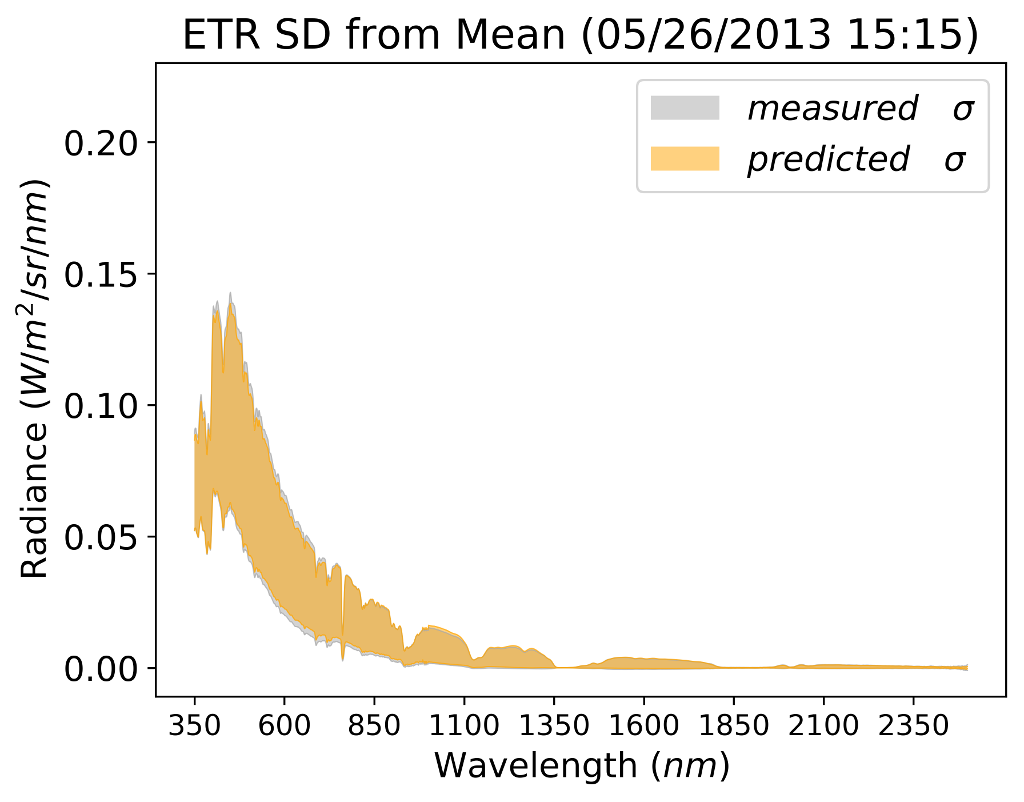
\includegraphics[width=0.32\textwidth]{img/model_etr_sd.png}
%\includegraphics[width=0.32\textwidth]{img/model_rfr_sd.png}
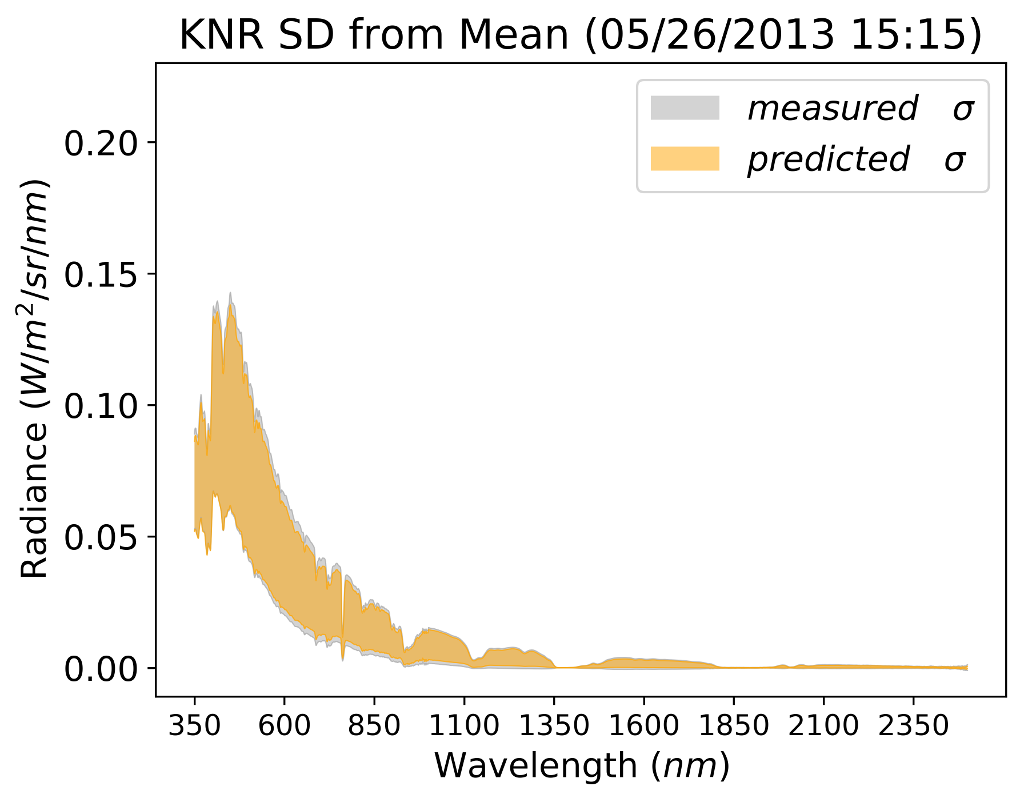
\includegraphics[width=0.32\textwidth]{img/model_knr_sd.png}
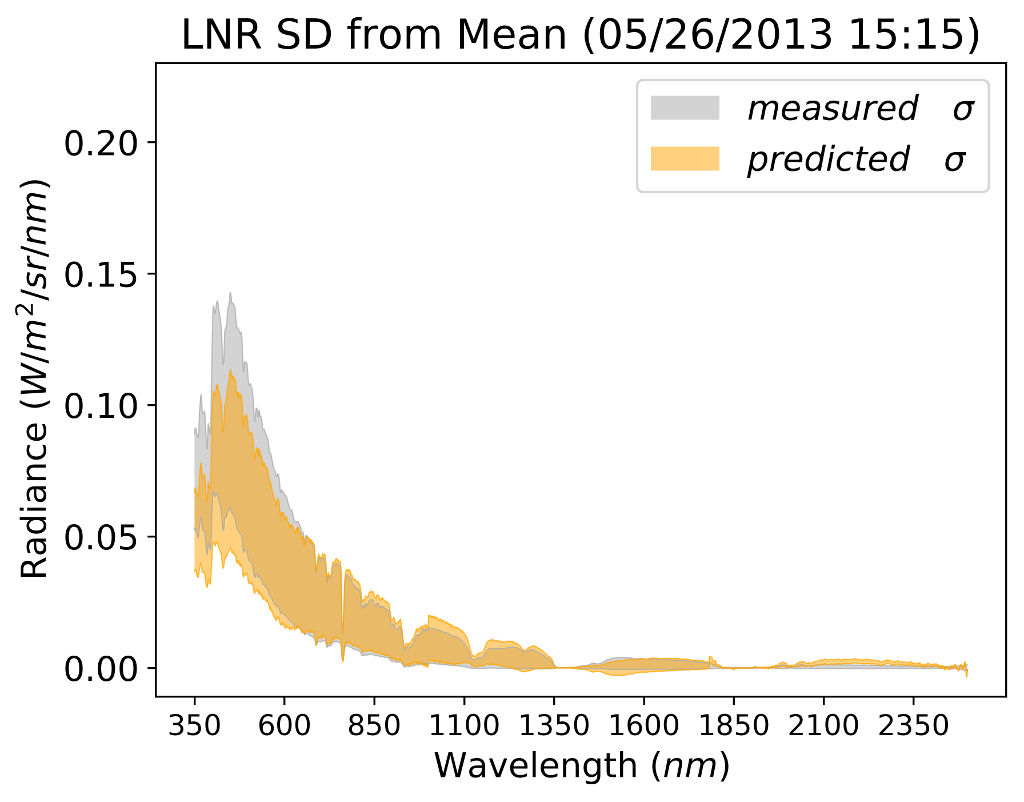
\includegraphics[width=0.32\textwidth]{img/model_lnr_sd.png}
\end{tabular}
\end{center}
\caption[prelimresults] { \label{fig:prelimresults}Three of the four final regression models, ETR, KNR, and LNR, respectively, showing measured and predicted standard deviation from mean on test capture 05/26/2013 15:15 (clear sky). RFR performed very similar to ETR.}
\end{figure}

\begin{table}[hbtp]
\caption[holdout]{Holdout error for final regression models using 10-fold cross validation training and testing over \textit{all usable test samples, across all skies} with train-test ratio of 3:1.\protect\footnotemark}
\label{tab:modelerror}
\centering      
\begin{tabular}{cl*{4}{c}}
    \\
    \toprule
    ID & \multicolumn{1}{c}{Name} & $\mathrm{R}^2$ & RMSD\\
    \midrule
    \rule[-1ex]{0pt}{3.5ex}  ETR & Extra Trees Regressor & 66.55\% & 82.62\% \\
    \rule[-1ex]{0pt}{3.5ex}  RFR & Random Forest Regressor & 62.84\% & 87.09\% \\
    \rule[-1ex]{0pt}{3.5ex}  KNR & K Neighbors Regressor & 58.57\% & 91.95\% \\
    \rule[-1ex]{0pt}{3.5ex}  LNR & Linear Regressor & 51.02\% & 99.99\% \\
    \bottomrule
\end{tabular}
\end{table}

\footnotetext{The high error was mostly due to scattered sky cover predictions, as shown in Sec. \ref{sec:results}}

\subsection{Sky Cover Models}
\label{sec:skycover}

After cross-validated training and testing of our conglomerate (``mix") dataset, with all usable training samples across all sky covers, we suspected that models trained on sky specific datasets might prove more effective. The feature importance graph in Fig.~\ref{fig:eda} confirms this. Thus we filtered the mix dataset into 3 additional datasets (clear, scattered, overcast) based on sky cover assessment (CLR, SCT, OVC, respectively), and divided each of them for CV training/testing and holdout validation testing with our final regression models. The mix dataset contained all usable samples and was almost 1GB in size. Training and testing on a smaller, more focused dataset should be computationally cheaper and possibly even more precise, since the training data better reflects the expected real-world data. As discussed in Sec. \ref{sec:data}, there are a variety of automated/procedural sky cover algorithms that could be employed in a real-time system to assess the input sky images to quickly determine which trained model to use for prediction.  One problem with this experiment was that clear, scattered, and overcast datasets contained 5548, 15508, and 1940 samples respectively (i.e. 24\%, 67\%, and 8\% of total usable samples), and thus overcast skies were not well represented.

